\section{Process Analysis}
\label{process-analysis}

The following section contains the aggregation of the requirements study.
It integrates the security review with the observations made at the obstetrics and gynaecology department at the \AMC{}.
What is described is the research process as observed by an outsider.

\paragraph{Research with the \projectdata{}}

When doing research in the medical domain a well known workflow is often used. Nwogu \cite{nwogu} has formally described and defined this workflow for scientific reporting purposes (\ie{} writing scientific papers).
The {\tt Research Workflow} in figure \ref{fig:research-workflow} shows the simplification of this workflow, which includes problem definition, formulation of research question, definition of methods, data acquisition, statistical analysis, analysis results, and drawing a conclusion.

Clinical research (\eg{} a trial) is well suited to follow this workflow, as each step can be executed in turn.
Of these steps data acquisition is often the most time-consuming part.
However, acquisition of new data is not always necessary,  desirable or even possible. 
Research data of high quality and trustworthiness is valuable and should be preserved and re-used, under well controlled conditions. 
This is also the case with the \projectdata{}.

For reuse purposes three actors are important: researcher, data manager, and interested third parties (\eg{} clinics, public, government).
Researchers are actors interested in analysis of the \projectdata{} for scientific ends.
The data manager is the central point of communication for everything that has to do with the dataset, but is also responsible for keeping an overview of everything that happens during the steps in the process.
Lastly, third parties are actors interested in research conclusions and possibly aggregated (statistical) data from the \projectdata{}.

Currently when a dataset like the \projectdata{} is exploited for reuse the following happens.
A researcher asks what data is available and can search to find what he/she needs.
Then the researcher formulates a data request and a permission granting process is initiated by the data manager.
A request contains the necessary information to base a permission decision on, \eg{} problem background, research question, perceived methods to answer question, and the requested data.
The research committee evaluates the request and based on this the researcher gets permission to receive data.

Observations and the security aspects made it clear that data requests had to be added to the system.
This differs from the initial assumption of a data management (\eg{} search, select, download) and analysis system.
The focus of the system shifted a little with the data request addition; however, it is still assumed that the main interest for the users will lie at the other functions.
The acquisition and analysis processes overspan a big chunk of the research workflow, which is depicted in figure \ref{fig:research-workflow} with the gateway function groups.

\begin{figure}[h]
	\centering
	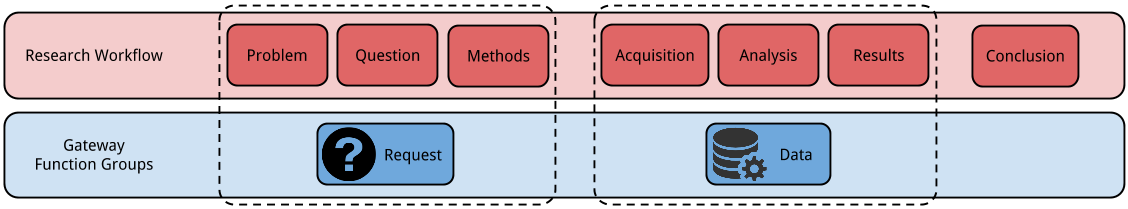
\includegraphics[width=1.0\linewidth]{images/research-workflow}
	\caption{
		Simplified research workflow often used  in the medical domain (based on Nwogu \cite{nwogu}).
		The workflow components are mapped  by the identified \ivfsystem{} function groups (dotted lines).
		%Note: the data acquisition component requires execution of acquisition methods defined in the methods component. \allard{remove note?}
	}
	\label{fig:research-workflow}
\end{figure}